\chapter{Vers une amélioration possible du support exécutif à travers la simulation}\label{chap:simulation}
\chaptertoc


Le chapitre~\ref{chap:contrib:characterization} a montré qu'il était possible de caractériser précisément à la fois les machines et les parties critiques d'applications vis à vis de ces machines.
Cela a pu confirmer et chiffrer l'importance de la localité des données sur les architectures NUMA.
Le chapitre précédent a montré comment nous avons étendu un modèle de programmation et les supports exécutifs pour mieux prendre en compte la localité des données, et globalement améliorer l'ordonnancement de l'application.

À partir de là, certaines questions peuvent se poser~: compte tenu des caractéristiques de l'application et des machines, peut on faire mieux ?
Si oui~: quelle marge reste-t'il à gagner par rapport aux ordonnancements théoriques connus ? Quelles caractéristiques faudrait il prendre en compte ?

%Dans le cadre spécifique de Cholesky, Agullo et al.\cite{Agullo2015} ont étudié les performances réelles de différentes stratégies d'ordonnancement dans StarPU, en ciblant des architectures hétérogènes, et en les comparant à une exécution simulée à travers SimGrid.
%Ils ont montrés que les exécutions simulées pouvaient s'approcher très prêt du maximum théorique de performances~; ils ont également montré que les performances réelles pouvaient se rapprocher de ce maximum théorique, en donnant plus d'informations (obtenues statiquement) au support exécutif à propos des tâches.
Le coût en temps d'un développement de nouvelles analyses ou stratégies dans les compilateurs et supports exécutifs peut être important, il est donc logique de se tourner vers la simulation.
Pour des architectures hétérogènes ou distribuées, plusieurs simulateurs existent déjà~: par exemple SimGrid~\cite{Casanova2001}, qui dispose d'une base d'utilisateurs importante, ou TaskSim~\cite{Rico2010}.
Stanisic et al.~\cite{Stanisic2015} ont étudié la simulation de supports exécutifs dynamiques à base de tâches sur des architectures hétérogènes.
Ils expliquent leur démarche pour porter StarPU par dessus SimGrid (et donc pouvoir émuler l'exécution du code réel), et présentent leurs résultats à la fois sur des architectures hétérogènes et sur des architectures NUMA.
Leur modélisation précise des communications vers les GPUs leur permettent d'obtenir des simulations très précises pour les architectures hétérogènes.
En revanche ils expliquent ne pas tenir compte des phénomènes NUMA pour des raisons de difficultés de modélisation~: ils montrent donc des simulations précises pour la taille d'un nœud, mais qui s'éloignent complètement de l'exécution réelle lors de l'utilisation de plusieurs nœuds.
À notre connaissance il n'y a pas eu plus de travaux sur SimGrid ou TaskSim concernant spécifiquement les architectures NUMA.
Nous avons donc développé un prototype de simulateur, dans le but de pouvoir apporter une réponse aux questions ci-dessus, sans pour autant impliquer de lourds développements logiciel.
% je pense que dans le papier il n'y a pas de modélisation des comms sur NUMA, vu que le cout de la tache est donné par la calibration starpu (et donc inclu la comm pour la mémoire partagée).

Ce chapitre est organisé de la façon suivante~: la section~\ref{sec:simulation:archi} décrit l'architecture générale du simulateur.
La section~\ref{sec:simulation:modeles} fait un point sur les différents modèles envisagés, et la section~\ref{sec:simulation:resultats} montre des résultats préliminaires obtenus avec ces modèles, en apportant des premières pistes de réponses aux questions posées.
Enfin la section~\ref{sec:simulation:next} décrit quels améliorations du simulateur seraient possible pour améliorer son réalisme.


\section{Fonctionnement du simulateur}\label{sec:simulation:archi}

\begin{figure}[h!]
  \centering
  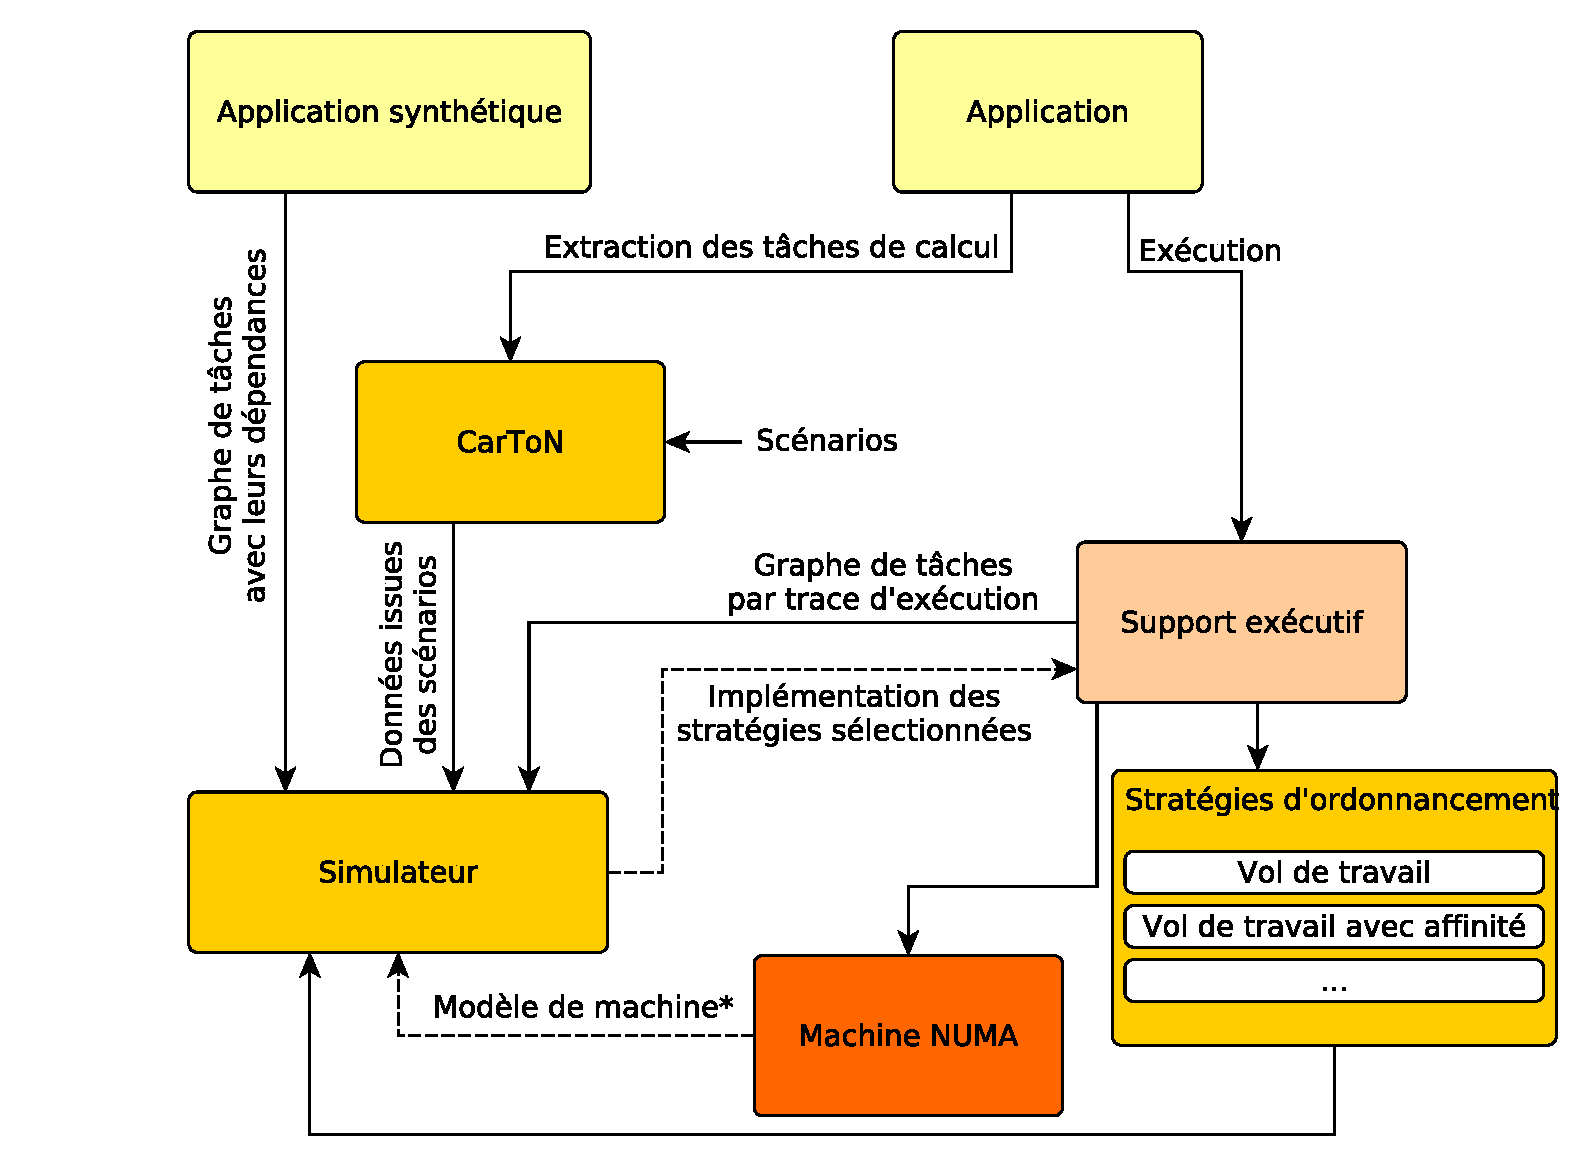
\includegraphics[width=\textwidth]{big_picture}
  \caption{Schéma d'interaction des différents programmes.\\ *~: partie envisagée mais encore non implémentée.}\label{fig:simu:big_picture}
\end{figure}

La figure~\ref{fig:simu:big_picture} illustre la place du simulateur par rapport aux autres travaux de cette thèse.
L'expression d'une application dans le simulateur se fait à travers une API dédiée.
Elle peut soit se faire directement à l'aide d'une trace d'une exécution réelle (obtenue via libKOMP), soit manuellement en décrivant l'application de manière synthétique.
Les coûts associés aux tâches peuvent être fournis au simulateur à l'aide de \outil.
La simulation a lieu en fonction du modèle d'architecture choisi et de la stratégie d'ordonnancement sélectionnée.

Le simulateur implémente un certain nombre de concepts que nous avons déjà abordés, détaillés ci-après.

\paragraph{Données~:} elles sont représentées comme des blocs de taille fixe, qui sont associés à un cœur lors de leur création (pour simuler la politique \emph{first-touch} du système d'exploitation).

\paragraph{Tâches~:} elles sont représentées de manière similaire à ce qui se fait dans les supports exécutifs.
Chaque tâche est composée d'une série d'actions séquentielles, pouvant être de trois types différents~:
\begin{itemize}
  \item \emph{READ}~: lecture d'un bloc de données
  \item \emph{WRITE}~: écriture d'un bloc de données
  \item \emph{COMPUTE}~: calcul avec un certain nombre d'instructions.
\end{itemize}

De plus des dépendances entre tâches peuvent être ajoutées en attachant un ensemble de prédécesseurs à une tâche donnée.

\paragraph{Topologie~:}
De manière similaire à ce que nous avons utilisé lors de nos travaux, nous avons considéré ici deux niveaux de hiérarchie, avec une file de tâche prêtes par cœur, et une file de tâche prêtes par nœud.

\paragraph{Ordonnancement~:}
L'objectif était de simuler le comportement d'un support exécutif similaire à ceux que nous avons utilisés dans le chapitre~\ref{chap:contrib:openmp}, nous avons donc basé l'ordonnancement au sein du simulateur sur du vol de travail.
Le moteur d'exécution repose sur deux fonctions \emph{steal} et \emph{push}, devant implémenter les processus de vol et de placement d'une tâche, respectivement.
Pour le besoin des premières comparaisons, nous avons implémenté deux heuristiques différentes, similaires à celles utilisées dans les résultats de la section~\ref{sec:contribs:perf_eval}~:
\begin{itemize}
  \item \emph{RandLoc}~: elle implémente un vol de travail aléatoire et un placement des tâches prêtes localement~; elle est équivalente à la combinaison de stratégies \emph{sRand/pLoc} décrites dans la section~\ref{sec:openmp:runtime:select}.
  \item \emph{Affinity}~: elle implémente un vol de travail hiérarchique et un placement des tâches conformément à l'affinité des données~; elle est équivalente à la combinaison \emph{sNumaProc/pNumaWLoc} décrite dans la section~\ref{sec:openmp:runtime:select}.
\end{itemize}


\paragraph{Modèle de l'architecture~:}

Un modèle fournit des informations cruciales~: il définit la topologie de la machine (nombre de cœurs, de nœuds, ainsi que les associations cœur/nœud), il défini également le coût de chaque opération (exprimé en secondes) en fonction de son type et du type de la tâche effectuant l'opération.

\section{Modèles de coût de tâches envisagés}\label{sec:simulation:modeles}

Le simulateur décompose le temps de chaque tâche de la manière suivante~:
$$
T_{tache} = \sum_{i} T_{lecture}(P_i) + T_{execution} + \sum_{i} T_{ecriture}(P_i)
$$

Où les $P_i$ sont les paramètres en lecture et écriture de la tâche.

Avant de modéliser précisément l'architecture, nous avons dans un premier temps décidé de considérer les tâches dans leur ensemble.
À travers \outil il est possible d'obtenir des temps d'exécution des tâches dans lesquels la totalité des opérations est pris en compte~; en jouant sur les conditions d'exécution il est donc possible d'obtenir les $T_{min}$ et $T_{max}$ observés, et borner le temps d'exécution d'une tâche~:
$$
T_{min} \leq T_{tache} \leq T_{max}
$$


Nous avons choisi de commencer à étudier l'application qui nous a servi de cas d'étude pour le chapitre~\ref{chap:contrib:characterization}~: Cholesky.
Les données récoltées à l'aide de \outil nous ont permis de comprendre précisément le comportement de chacun des quatre noyaux impliqués dans la factorisation de Cholesky.
En particulier nous avons les $T_{min}$ et $T_{max}$ de chaque noyau en fonction de la charge de la machine, et le $T_{tache}$ moyen en fonction du type d'accès aux données (local ou distant).

Nous avons implémenté un Cholesky synthétique correspondant à l'algorithme de l'application dans le simulateur, et considéré plusieurs modèles de coûts afin d'évaluer le simulateur et éventuellement les bornes de l'application en terme de performances.

\begin{table}[t!]
\def\arraystretch{1.5}
\centering
\begin{tabular}{|c||c|c|c|}\hline
  \multirow{2}{*}{Noyau} & \multirow{2}{*}{\makecell{Nombre d'exécution concurrentes\\(threads)}} & \multicolumn{2}{c|}{\makecell{Performance moyenne\\par cœur (GFLOPS)}} \\ \cline{3-4}
    & & Données locales & Données distantes \\ \hline
  \multirow{2}{*}{\potrf}
    & 1 & 11.48 & 11.66 \\ \cline{2-4}
    & 8 & 11.08 & 11.11 \\ \cline{2-4}
    & 192 & 9.30 & 8.81 \\ \cline{2-4}
  \hline
  \multirow{2}{*}{\trsm}
    & 1 & 14.20 & 14.38 \\ \cline{2-4}
    & 8 & 13.19 & 12.22 \\ \cline{2-4}
    & 192 & 10.00 & 9.15 \\ \cline{2-4}
  \hline
  \multirow{2}{*}{\syrk}
    & 1 & 16.14 & 16.41 \\ \cline{2-4}
    & 8 & 13.97 & 13.59 \\ \cline{2-4}
    & 192 & 10.10 & 7.51 \\ \cline{2-4}
  \hline
  \multirow{2}{*}{\gemm}
    & 1 & 16.92 & 17.10 \\ \cline{2-4}
    & 8 & 16.32 & 14.11 \\ \cline{2-4}
    & 192 & 14.45 & 12.82 \\ \cline{2-4}
  \hline
\end{tabular}
\caption{Tableau illustrant les performances réelles (en GFLOPS) des noyaux de Cholesky sur des matrices de taille 512, sur idchire}\label{tab:simu:perf-kernels-idchire}
\end{table}

Afin de pouvoir illustrer les différents modèles de coût que nous avons testés, le tableau~\ref{tab:simu:perf-kernels-idchire} regroupe quelques exemples de performance pour les noyaux de Cholesky, pour une taille de matrice de 512, en fonction de la charge de la machine (comme décrit dans la section~\ref{sec:contribs:apps:cholesky:scenario}) et du type d'accès.

Cet aperçu des performances permet de montrer que si la localité des données n'a pas d'impact positif pour un unique thread, à partir du moment où tous les threads d'un nœud sont utilisés (et donc a fortiori en pleine charge) la différence de performance est significative.

Nous avons donc dégagé plusieurs modèles de coûts des tâches.
Ces modèles se basent sur les expériences que nous avons pu faire avec \outil.
Au cours de ces expériences, nous avons fait varier deux paramètres qui peuvent avoir un impact majeur sur les performances~: l'emplacement des données du noyau, et la charge de la machine.
En faisant varier ces deux paramètres de manière extrème, nous avons pu obtenir un profil a priori complet des noyaux, pour nourir les modèles de coût ci-dessous.

\paragraph{Modèle "Minimum"~:} ce modèle a pour but d'estimer la performance minimum que l'on est a priori en droit d'attendre d'un support exécutif implémentant une stratégie de vol de travail naïve.
Pour se faire, nous avons considéré seulement la performance minimale de chacun des noyaux pour le coût de chaque tâche, parmi les expériences que nous avions effectuées avec \outil.
En pratique cela correspond à un cas extrème pour l'emplacement des données~: toutes les données à distance, et à une charge complète de la machine.
En terme de scénario, sur idchire, cela revient à exécuter 192 noyaux simultanément, avec leurs données placées sur un nœud distant, de manière similaire à ce que nous avons effectué pour la figure~\ref{fig:contribs:apps:cholesky:perf-512-remote-idchire}.

\paragraph{Modèle "Maximum"~:} à l'inverse l'objectif de ce modèle est de donner une borne supérieure pour les performances du support exécutif.
Nous avons donc considéré seulement la performance a priori maximale de chacun des noyaux pour le coût de chaque tâche.
Cela correspond à l'autre extrème en terme de distribution de données~: toutes les données locale, et à une exécution non perturbée par d'autres noyaux.

\paragraph{Modèle "DeuxNiveaux"~:} l'objectif de ce modèle est d'essayer de simuler au plus près le comportement des noyaux, en utilisant deux niveaux de coût~: soit celui correspondant à l'exécution avec des données locales, soit celui correspondant à l'exécution avec des données distantes.
La simulation étant lancée sur un nombre de cœurs connus, nous avons utilisé les performances de référence des noyaux correspondant à la charge de la machine simulée, que nous avons obtenues à travers les scénarios exécutés par \outil.
Lors de la simulation nous déterminons si les accès en écriture de la tâche sont locaux ou distant, et le coût de la tâche correspondante est utilisé.




\section{Résultats préliminaires}\label{sec:simulation:resultats}


Nous avons commencé par comparer les modèles entre eux.
Pour ce faire nous avons choisi un cas réel ou l'affinité avait un impact significatif~: une taille de bloc de 512 pour une taille de matrice de 32768, avec des blocs de données répartis de manière cyclique sur la machine.
Les résultats des simulations avec les différents modèles sont montrés sur la figure~\ref{fig:simu:modeles:idchire}.

\begin{figure}[h!]
  \centering
  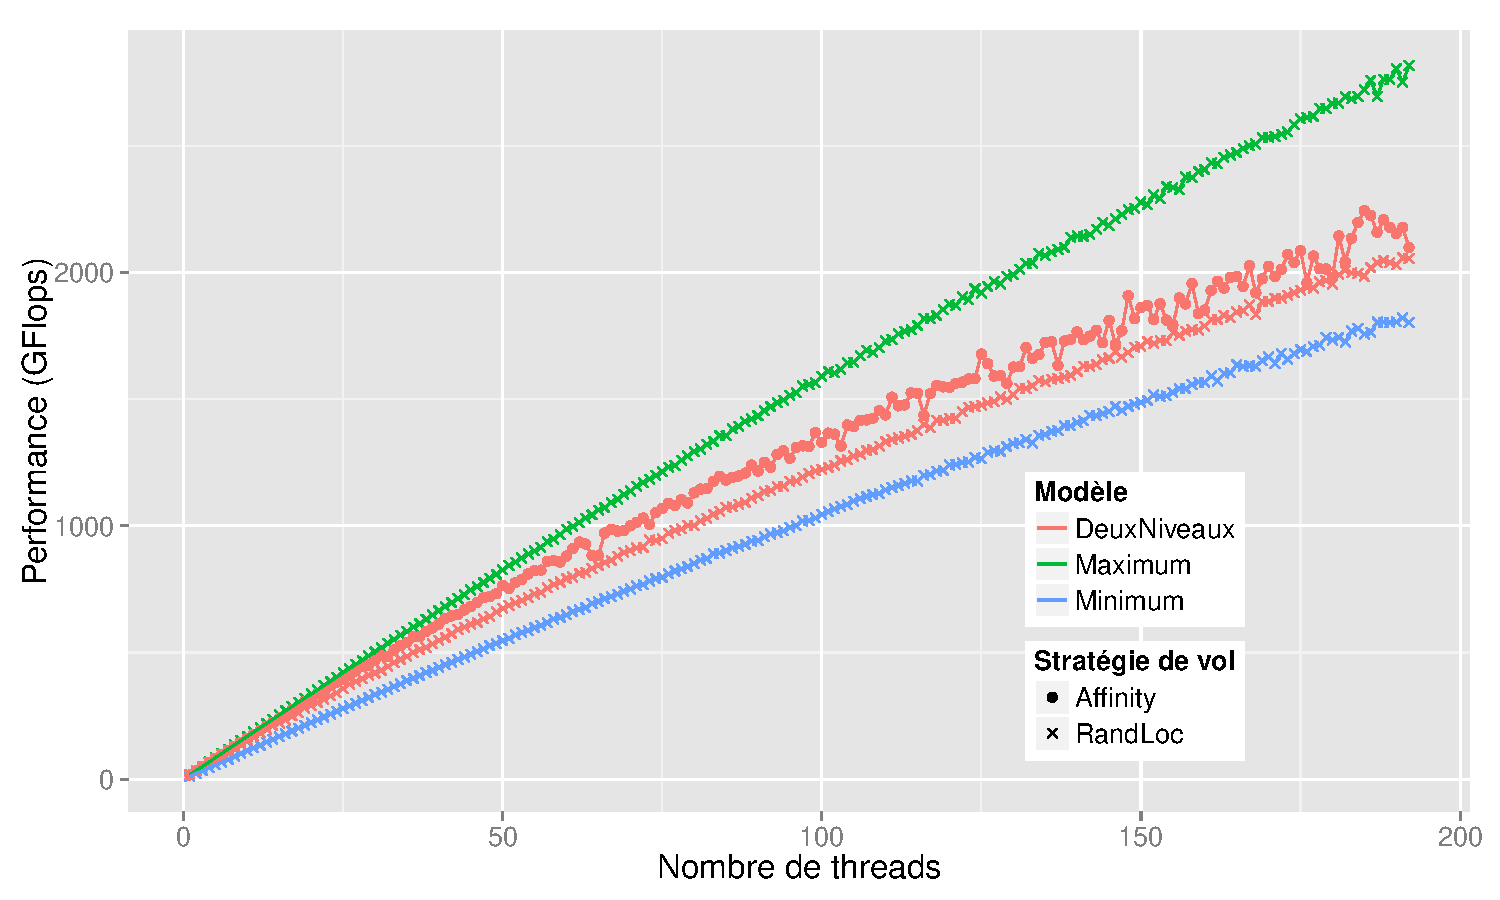
\includegraphics[width=\textwidth]{simu_min_max_affinity_idchire}
  \caption{Comparaison des différents modèles et stratégies, basés sur les références d'idchire. Taille de bloc~: 512, taille de matrice~: 32768}\label{fig:simu:modeles:idchire}
\end{figure}


Les premières observations à faire sur cette figure sont plutôt positives~: les performances affichées semblent réalistes, le modèle \emph{DeuxNiveaux} est correctement encadré par les modèles \emph{Minimum} et \emph{Maximum}, et au sein du modèle \emph{DeuxNiveaux}, il y a bien une différence claire entre un vol de travail <<naïf>> --- \emph{RandLoc} --- et un vol de travail hiérarchique et sensible à l'affinité --- \emph{Affinity}.

\begin{table}[h!]
\def\arraystretch{1.5}
\centering
\begin{tabular}{|c||c|c|c|c|}\hline
  \multirow{2}{*}{Stratégie} & \multicolumn{2}{c|}{Lectures} & \multicolumn{2}{c|}{Écritures} \\ \cline{2-5}
    & Locales & Distantes & Locales & Distantes \\
  \hline
  \emph{RandLoc} & 4 380 & 117 066 & 1902 & 43 858 \\
  \hline
  \emph{Affinity} & 15 343 & 88 045 & 22 556 & 23 204 \\
  \hline
\end{tabular}
\caption{Nombre de lectures et écritures de blocs locaux ou distants en fonction de la stratégie de vol}\label{tab:simu:acces-blocs-idchire}
\end{table}

Cela est confirmé en regardant le nombre de lectures et écritures locales ou distantes, rapportées dans le tableau~\ref{tab:simu:acces-blocs-idchire}.
Ce tableau montre que le nombre d'accès distants est significativement diminué par l'utilisation d'une stratégie de vol de travail sensible à l'affinité~: le nombre d'écritures distantes est réduit de moitié, tandis que le nombre de lectures distantes est réduit d'environ 25\%.


\begin{figure}[t!]
  \centering
  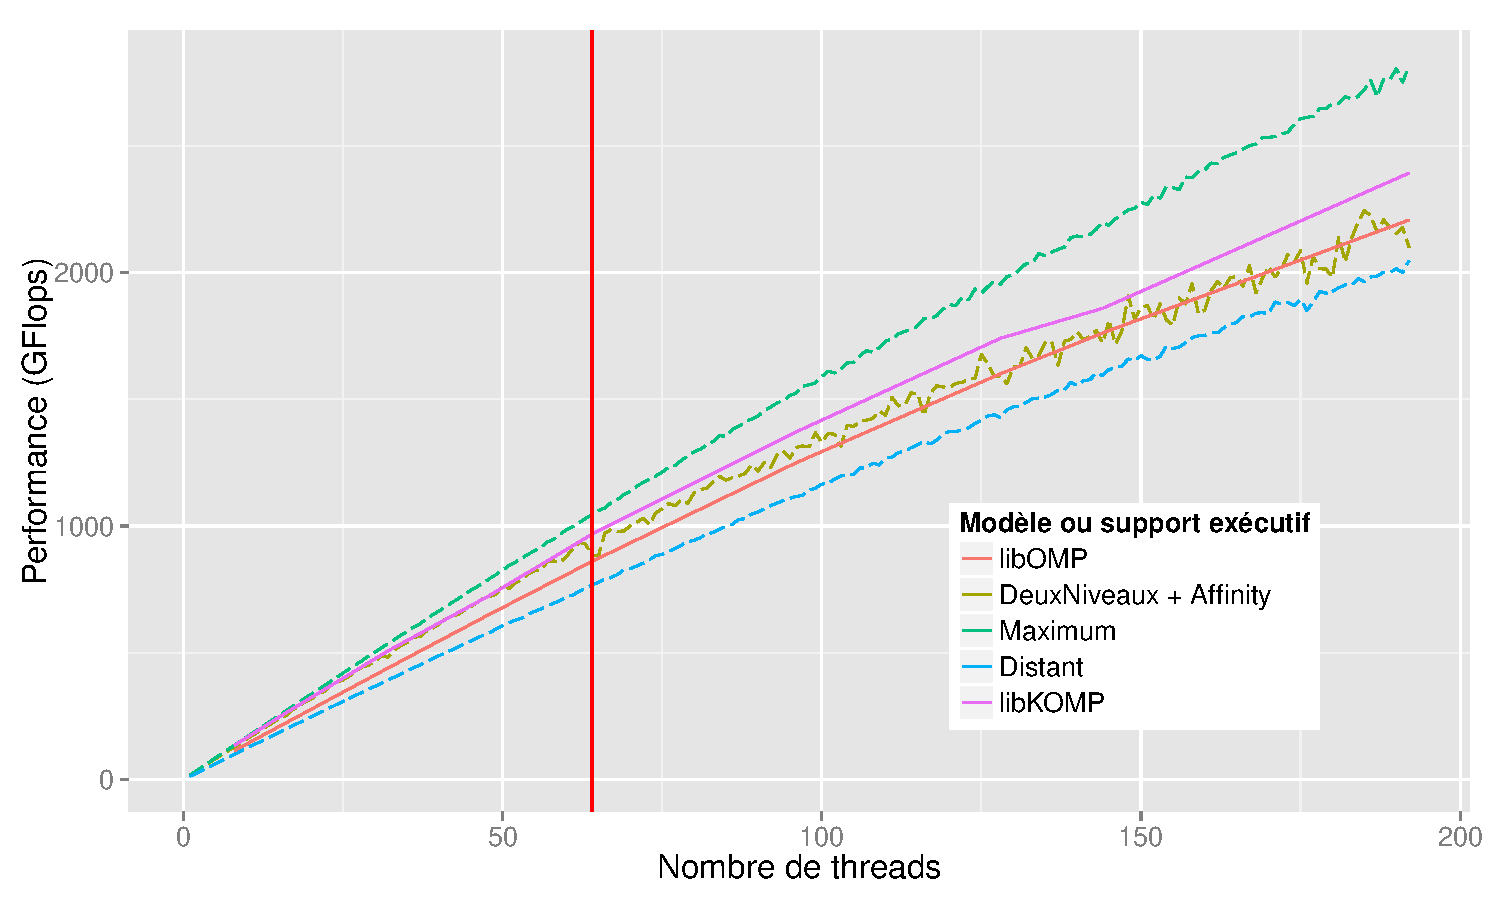
\includegraphics[width=\textwidth]{simu_affinity_runtime_idchire}
  \caption{Comparaison des certains modèles aux supports exécutifs sur idchire, pour une taille de matrice de 32768 et une taille de bloc de 512}\label{fig:simu:modeles-vs-runtime:idchire}
\end{figure}
%\begin{figure}[h!]
  %\centering
  %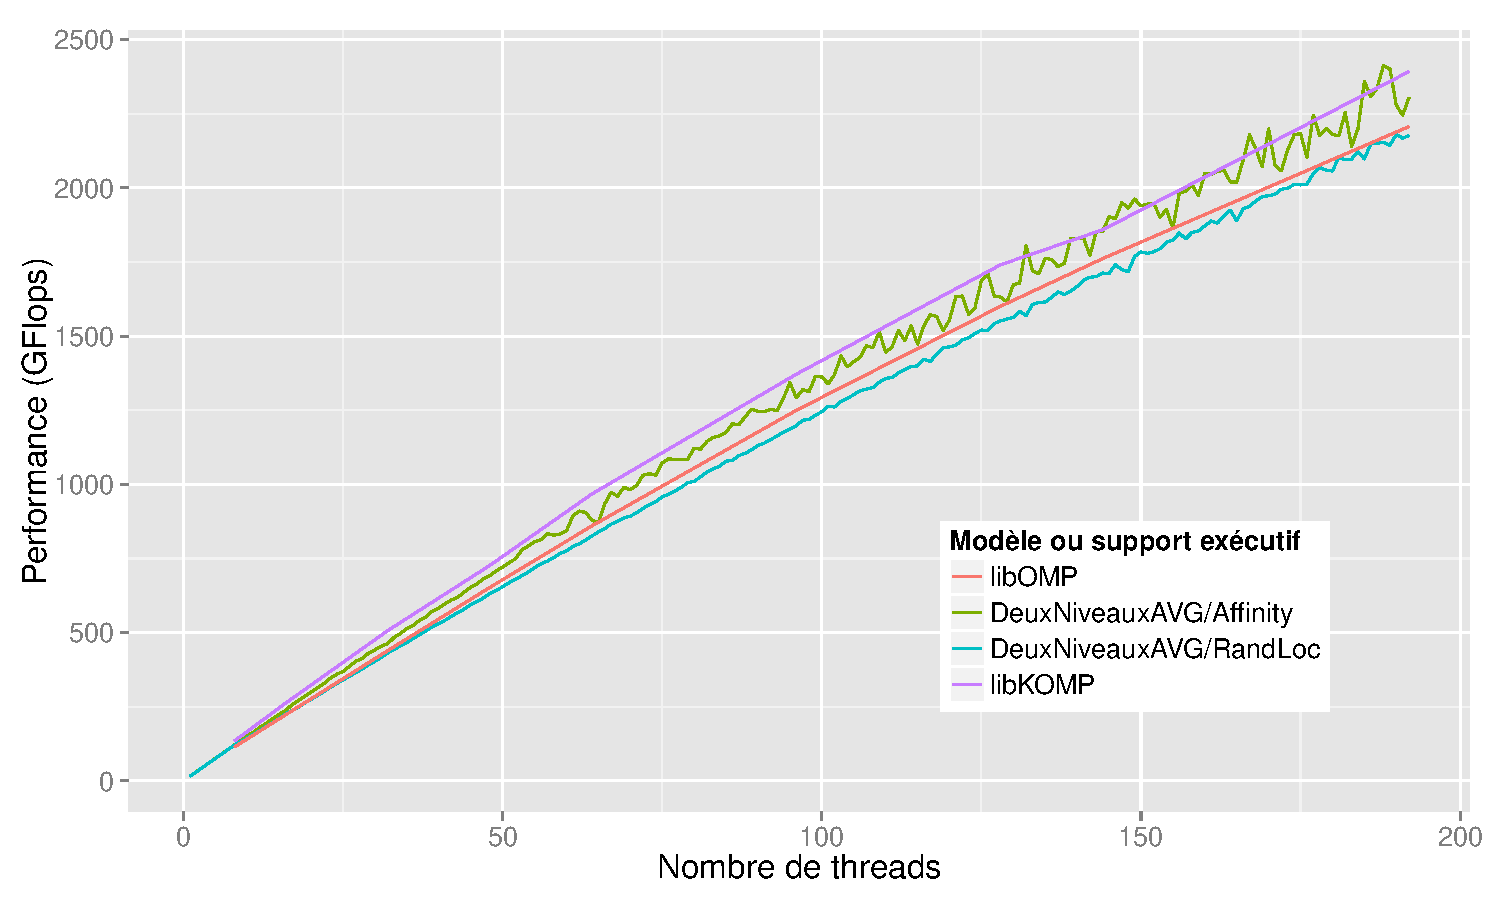
\includegraphics[width=\textwidth]{simu_affinity_avg_runtime_idchire}
  %\caption{Comparaison du modèle \emph{DeuxNiveauxAVG} aux supports exécutifs sur idchire, pour une taille de matrice de 32768 et une taille de bloc de 512}\label{fig:simu:affinityavg-vs-runtime:idchire}
%\end{figure}


Ces figures sont bien sur issues de simulation~; que valent elles en comparaison aux chiffres obtenus à travers les expériences ?
La figure~\ref{fig:simu:modeles-vs-runtime:idchire} compare les modèles \emph{Minimum} (avec vol aléatoire) et \emph{DeuxNiveaux} (avec vol hiérarchique) aux supports exécutifs libOMP (qui utilise un vol aléatoire) et libKOMP (qui utilise un vol hiérarchique et l'affinité).
Comme on peut le constater, les performances des deux supports exécutifs sont effectivement supérieures au minimum simulé. En revanche les performances simulées de l'affinité semblent légèrement en retrait compte tenu des performances réelles.

Cette différence pourrait sembler étonnante, mais pourrait être en partie expliquée par le fait que les performances de référence ont été obtenues lorsque les données étaient soit \textit{toutes} locales ou \textit{toutes} distantes.
Alors que dans la réalité il peut évidemment y avoir plusieurs autres cas quand plusieurs blocs sont en paramètre des noyaux.
Cela donnerait donc une version <<minimum>> des performances plus pessimistes que la réalité.
Ces travaux étant en cours, plusieurs pistes d'amélioration sont envisagées, et sont décrites dans la section~\ref{sec:simulation:next}.


%Nous avons essayé de prendre la moyenne globale des performances de chaque noyau comme référence, sous le modèle \emph{DeuxNiveauxAVG}.
%Les résultats obtenus sont présentés sur la figure~\ref{fig:simu:affinityavg-vs-runtime:idchire}.

%La simulation des deux heuristiques semblent adhérer un peu mieux à la réalité, bien qu'il semble possible de gagner encore en précision.


Les résultats obtenus sur les cas favorable à l'utilisation de l'affinité sont assez encourageants.
Nous avons également appliqué la simulation sur des tailles de bloc plus petites, typiquement pour une taille de matrice de 8192 avec des blocs de 256.

\begin{figure}[h!]
  \centering
  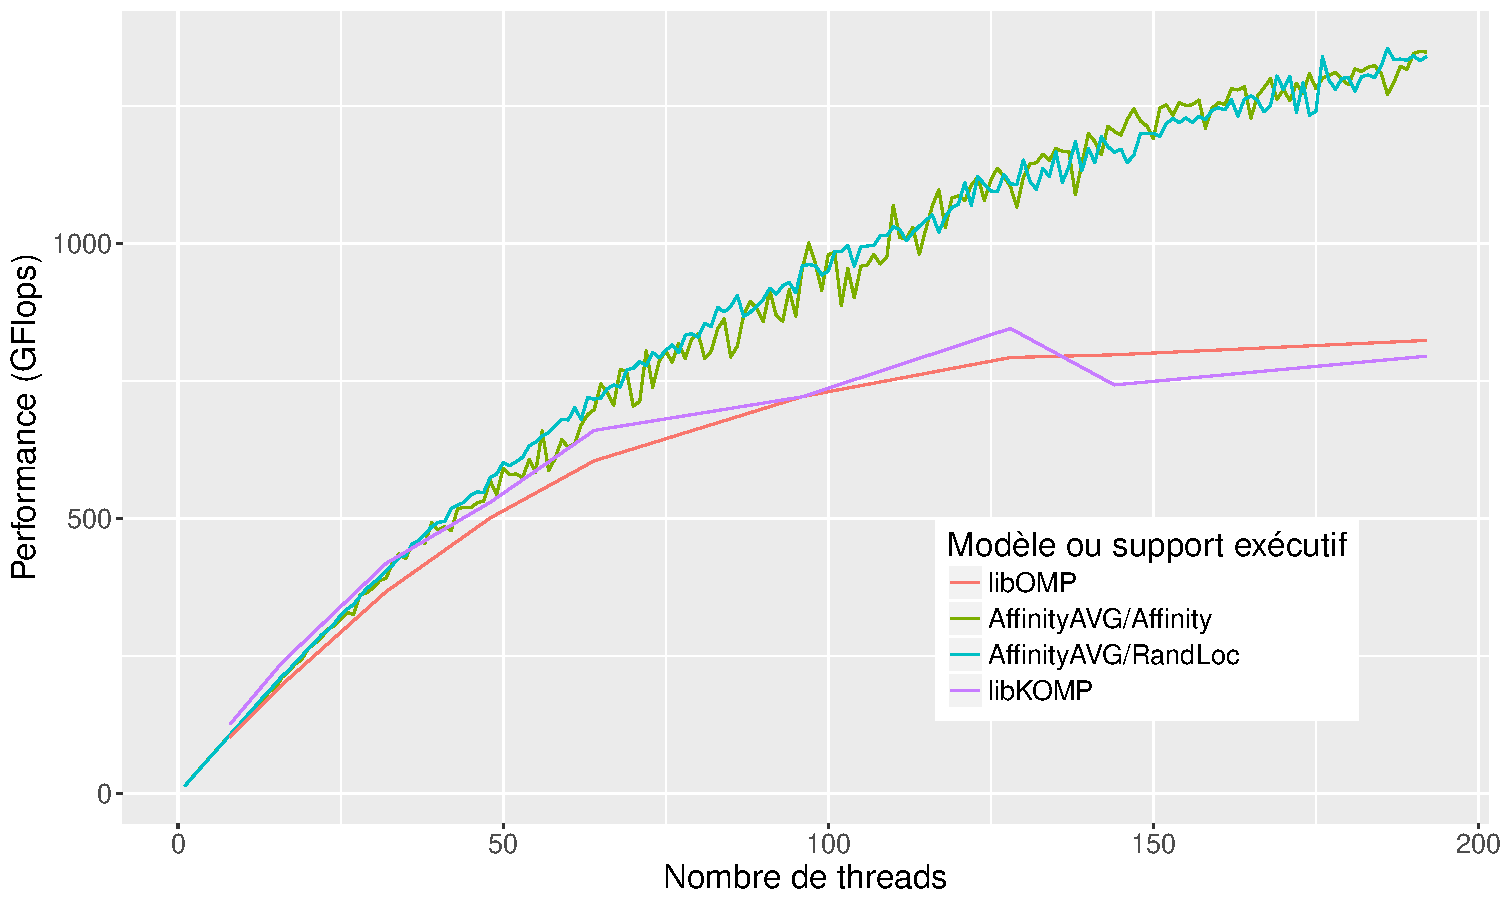
\includegraphics[width=\textwidth]{simu_affinity_8k_runtime_idchire}
  \caption{Comparaison du modèle \emph{DeuxNiveaux} aux supports exécutifs sur idchire, pour une taille de matrice de 8192 et une taille de bloc de 256}\label{fig:simu:affinityavg-8k-vs-runtime:idchire}
\end{figure}

%# --------------- Explicit task
%#                                            <task name>    <count>   Work (sum/avrg/sd)
% init      11264   1.9237e+02   1.7078e-02   2.6301e-04
% dpotrf        352   3.9004e-01   1.1081e-03   1.9407e-04
% dtrsm       5456   1.6495e+01   3.0232e-03   1.2368e-04
% dsyrk       5456   1.5825e+01   2.9006e-03   1.7507e-04
% dgemm      54560   1.9441e+02   3.5633e-03   3.7560e-05
% FLOPS pour bloc 256
% dpotrf : 5.62522e+06
% dtrsm : 1.67772e+07
% dsyrk : 1.68428e+07
% dgemm : 3.35544e+07
% soit en flops moyen :
% dgemm : 9.41 gflops
% dtrsm : 5.55 gflops
% dsyrk : 5.80 gflops
% dpotrf : 5.07 glops


Les résultats obtenus sont présentés sur la figure~\ref{fig:simu:affinityavg-8k-vs-runtime:idchire}.
Comme on a pu le constater sur les expériences réelles, la simulation ne montre également aucune différence de performances avec ou sans l'utilisation de l'affinité.

En revanche, passé un certain nombre de cœurs, les performances des deux supports exécutifs sont assez loin de celles a priori atteignables !
Le nombre de tâches dans une telle configuration peut vite limiter le parallélisme exposé, ce qui va donc entrainer une augmentation importante du nombre de requêtes de vol émises par les threads inactifs.

\begin{figure}[h!]
  \centering
  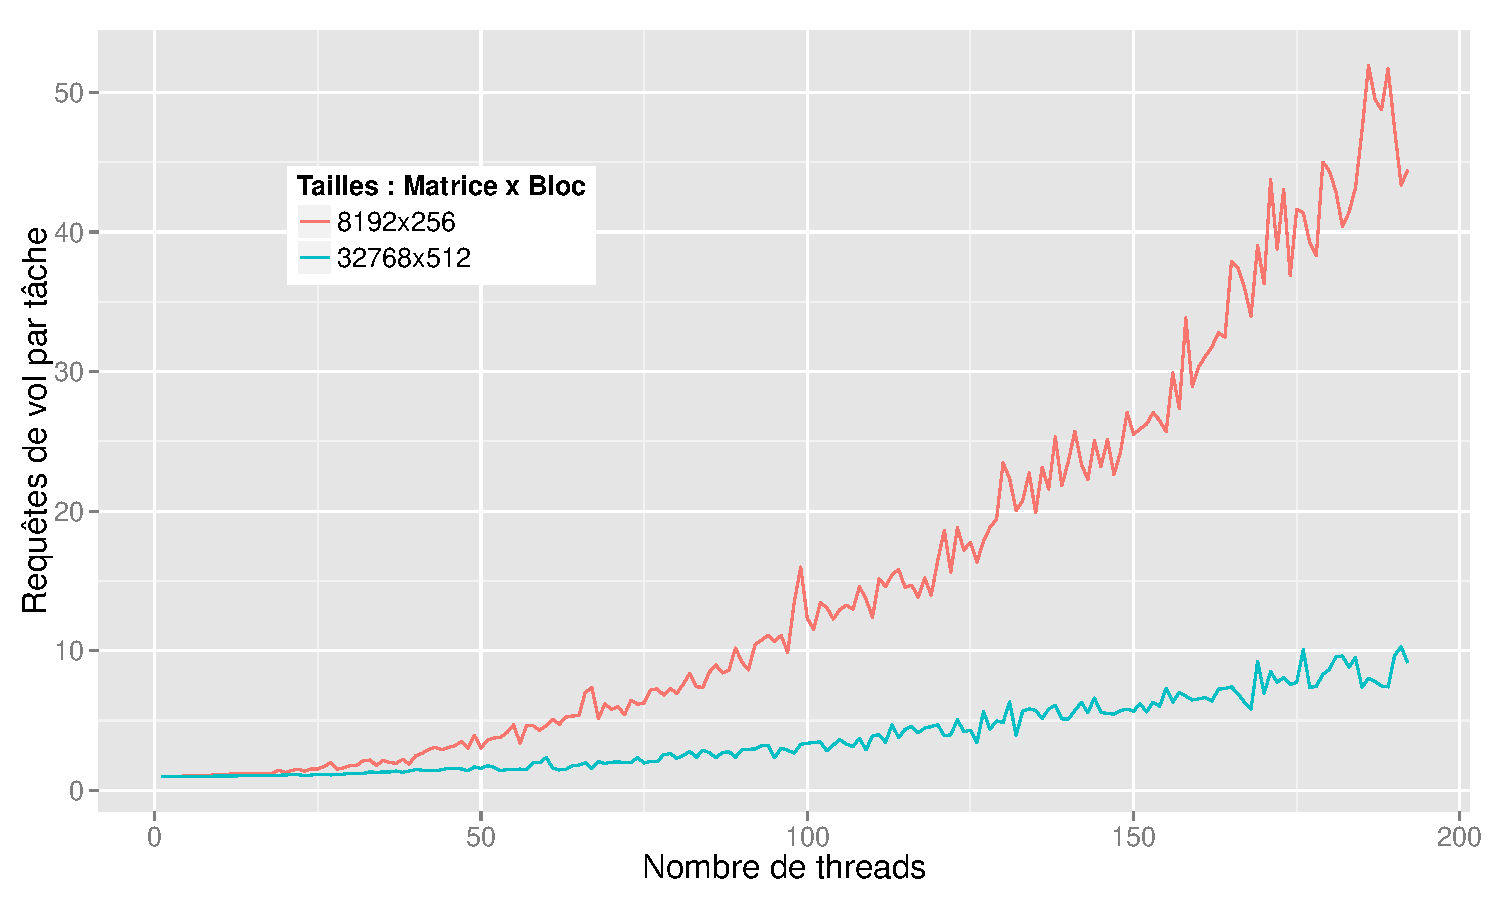
\includegraphics[width=\textwidth]{simu_steal_visits_idchire}
  \caption{Comparaison de l'évolution du nombre de requêtes de vol par tâche dans le simulateur, en fonction de la taille de matrice}\label{fig:simu:steals_per_task:idchire}
\end{figure}

Ce phénomène est illustré sur la figure~\ref{fig:simu:steals_per_task:idchire}, où l'on voit l'évolution du nombre de requêtes de vol divisé par le nombre de tâches à exécuter, au sein du simulateur.
Pour un cas exposant un fort parallélisme, une taille de matrice de 32768 avec une taille de bloc de 512 et donc plus de 45000 tâches, on peut constater que le nombre de requêtes par tâche reste raisonnable.
En revanche pour le cas étudié dans la figure~\ref{fig:simu:affinityavg-8k-vs-runtime:idchire}, une taille de matrice de 8192 avec une taille de bloc de 256 et donc un peu moins de 6000 tâches, on peut constater une 'évolution du nombre de requêtes de vol par tâche est exponentielle, et qu'il pourrait y avoir une corrélation entre le nombre de requêtes et l'impact sur les performances.

\begin{table}[t!]
\def\arraystretch{1.5}
\centering
\begin{tabular}{|c||c|c|}\hline
  Noyau & \makecell{Performance minimum attendue\\(GFlops)} & \makecell{Performance moyenne observée\\(GFlops)} \\
  \hline
  \potrf & 5.88 & 5.07 \\
  \hline
  \trsm & 7.22 & 5.55 \\
  \hline
  \syrk & 7.51 & 5.80 \\
  \hline
  \gemm & 11.61 & 9.41 \\
  \hline
\end{tabular}
\caption{Comparaison des performances minimum attendues aux performances moyennes observées pour l'exécution de Cholesky sur 192 cœurs, avec une taille de matrice de 8192 et des blocs de taille 256}\label{tab:simu:comparaison-modele-observation}
\end{table}


Pour une taille de matrice de 8192 (taille de bloc 256) et avec 192 cœurs, nous avons observés les temps moyens passés dans chaque tâche, rapportés par les traces de libKOMP.
Nous les avons comparé aux performances minimum considérées par le simulateur dans le tableau~\ref{tab:simu:comparaison-modele-observation}.

Nous avons constaté une forte différence entre les performances réelles et les coûts de tâches considérés par le simulateur.
La différence observée sur la figure~\ref{fig:simu:affinityavg-8k-vs-runtime:idchire} ne semble donc pas venir d'un surcoût d'exécution du support exécutif lié à la quantité de requêtes de vol exécutées.
En revanche les requêtes de vol peuvent générer du trafic sur les bus mémoires~: non seulement les threads ne participent plus activement à l'exécution du programme, mais en plus ils peuvent participer à la saturation de la bande passante et donc dégrader les performances des threads actifs.
Cela pourrait expliquer en partie la différence observée dans le tableau~\ref{tab:simu:comparaison-modele-observation}, et pourrait être prise en compte lors de la modélisation des coûts de communication.

Cela signifie également qu'il faudrait revoir la manière dont nous avons construit les coût pour le modèle \emph{Minimum}~: la charge maximale de la machine consiste en des noyaux s'exécutant indépendamment, il faudrait ici utiliser \outil pour venir ajouter une perturbation réaliste sur les ressources utilisées, afin de retrouver un pire cas d'exécution tel que constaté dans le tableau~\ref{tab:simu:comparaison-modele-observation}.

\subsection*{Évaluation du temps de simulation}

Un autre avantage de la simulation est qu'il n'y a pas besoin d'exécuter réellement les noyaux d'exécution, seulement de considérer le temps qu'ils prendraient.
Bien qu'une étude détaillée n'ait pas été réalisée, le temps nécessaire pour simuler les plus gros cas (comme la figure~\ref{fig:simu:modeles-vs-runtime:idchire}) est de seulement quelques secondes, contre plusieurs heures qui seraient nécessaires pour générer les même courbes.


%\section{Application d'un ordonnancement théorique}\label{sec:simulation:theorie}

%ref model:

%\cite{Pan2014}, Modeling cache coherence misses on multicores

%\cite{Stanisic2016}, Fast and Accurate Simulation of Multithreaded Sparse Linear Algebra Solvers

%\begin{todo}
%GRAPHE : courbes Julien sur Cholesky sélectionnés

%+mettre la section dans un endroit approprié, probablement après la description du modèle histoire de dire "ça c'est ce qu'on peut faire au mieux".
%\end{todo}

\section{Discussions et améliorations possibles}\label{sec:simulation:next}

Nos travaux sur la simulation sont très récents et encore en cours de développement.
Afin de généraliser la portée du simulateur et améliorer sa précision, nous évoquons ici les différentes pistes en cours d'étude.

\subsection{Modélisation du cache L3}

La version actuelle du simulateur inclu un cache par cœur de taille infinie.
Ce cache est modélisé comme une liste de blocs, dans une \emph{version} particulière.
À chaque écriture du bloc, la version du bloc est incrémentée.
Si une tâche effectue une lecture de ce bloc et que sa version correspond à la version du cache, alors la lecture ne coûte rien, sinon le cout de lecture est demandé au modèle.

Comme indiqué dans les sections précédentes, les modèles envisagés pour l'instant se basent uniquement sur le cout global d'une tâche, plutôt que sur des actions séparées.

L'une des améliorations nécessaires pour augmenter la précision du modèle serait l'introduction d'un cache partagé entre les cœurs d'un même nœud, disposant d'une capacité définie par le modèle, et implémentant une politique d'éviction relativement proche de celle utilisée par le matériel~: \emph{LRU}.

\subsection{Modélisation de la bande passante}

Le chapitre~\ref{chap:contrib:characterization} nous a permis d'étudier en détail le comportement de nos deux machines expérimentales.
Les figures~\ref{fig:contribs:machines:idchire:saturation} et~\ref{fig:contribs:machines:idchire:saturation-output} permettent de conclure par exemple que la bande passante d'idchire se comporte d'une manière assez proche d'un modèle de réseau limité.
L'objectif serait donc d'introduire un coût d'accès aux blocs mémoires suivant ce modèle.

\subsection{Modélisation de l'impact des requêtes de vol}

Nous avons observé une différence très importante entre la simulation et l'exécution réelle sur la figure~\ref{fig:simu:affinityavg-8k-vs-runtime:idchire}.
La figure~\ref{fig:simu:steals_per_task:idchire} et le tableau~\ref{tab:simu:comparaison-modele-observation} ont permis de déduire deux choses~: il pourrait y avoir une corrélation entre le nombre de requêtes de vol et la différence de performance observée, mais elle n'est pas due à un surcoût dans le support exécutif.
Ces requêtes de vol sont due au parallélisme limité des cas étudiés, et elles peuvent contribuer à la saturation de la bande passante.

Il faudrait donc pouvoir estimer l'impact des requêtes de vol sur le trafic mémoire.
Cela semble assez compliqué à exprimer à l'aide d'un scénario de \outil, mais cela pourrait sûrement se faire au sein de libKOMP~: il devrait être possible de faire exécuter des tâches sur les threads d'un unique nœud via une affinité stricte, et d'augmenter progressivement le nombre de requêtes de vols en ajoutant des threads en dehors de ce nœud (qui ne pourrait pas voler de tâche avec succès à cause de l'affinité stricte).


\subsection{Optimisation de la distribution}

Le simulateur permet d'obtenir des informations précises sur la distribution de données et son impact sur les accès locaux et distants.
Comme on l'a vu dans le tableau~\ref{tab:simu:acces-blocs-idchire}, le vol de travail respectant l'affinité permet de réduire considérablement les accès distants.
Il devrait donc être possible d'utiliser le simulateur pour automatiquement trouver la <<meilleure>> distribution de données (c'est à dire celle qui minimise les accès distants), en se basant sur une distribution cyclique et en introduisant des paramètres tels que le premier nœud considéré, le nombre de blocs alloués en même temps, et le pas lors du parcours des nœuds.
